\documentclass{amsart}
\usepackage{amsaddr}
\usepackage{listings}
\usepackage{times}
\usepackage[italic]{mathastext}
\usepackage{enumerate}
\usepackage{graphicx}

% default figure size
\setkeys{Gin}{width=0.6\linewidth, keepaspectratio}

% title, author, etc.
\title[Ch. 2: Simple Linear Regression]{Solutions to\\Chapter 2: Simple Linear Regression}
\author{Connor K. Brubaker}
\address{Department of Statistics\\Texas A\&M University}

% listings setting
\lstset{
    basicstyle=\footnotesize\ttfamily
}

\begin{document}
    \maketitle
    \section*{Problem 1}
    We begin by reading in the data and fitting a simple linear regression model to the data using the code below.
    \lstinputlisting[linerange={2-3}]{R/2.1_playbill.R}
    \begin{enumerate}[(a)]
        \item Use the code below to find the desired confidence interval for the slope $\beta_1$.
        \lstinputlisting[linerange={6-11}]{R/2.1_playbill.R}
        As we see from the output, the 95\% confidence interval for $\beta_1$ is $(0.9515, 1.0127)$. Since the value $1$ is included in this interval, we can say $1$ is a plausible value for the slope $\beta_1$.
        
        \item Use the code below to find the test statistic and $p$-value for this hypothesis test.
        \lstinputlisting[linerange={14-19}]{R/2.1_playbill.R}
        Assuming a significance level of $\alpha = 0.05$, we fail to reject the null hypothesis that $\beta_0 = 10000$. We cannot say we have signifiacnt enough evidence to argue that the intercept differs from \$10,000. 

        \item Use the code below to find the 95\% prediction interval for $x^* = 400000$.
        \lstinputlisting[linerange={22-26}]{R/2.1_playbill.R}
        Because the value \$450,000 falls outside the prediction interval, it is not a feasible value for the gross box office results in the current week when the previous week gross box office results were \$400,000. 

        \item The code below produces the plot in Figure \ref{fig:playbill_d}. 
        \lstinputlisting[linerange={30-43}]{R/2.1_playbill.R}
        The red dashed lines in this plot give 95\% prediction intervals for each value of \texttt{LastWeek} in the data set. The blue solid line represents the line $y = x$. Given that the blue line falls entirely within the bands of the prediction interval, I would argie that the prediction rule described in the problem statement is appropriate.
    \end{enumerate}

    \begin{figure}
        \centering 
        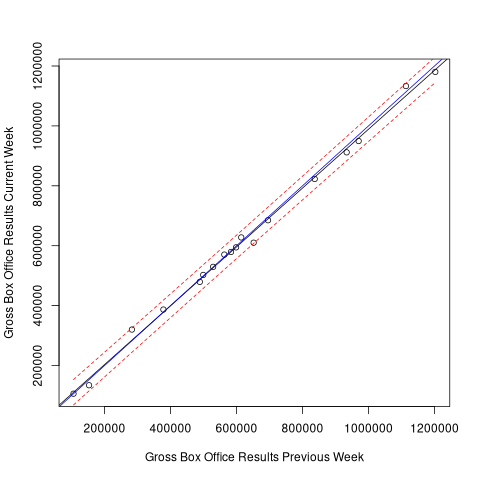
\includegraphics[]{figures/playbill_d.png}
        \caption{Prediction interval plot for Problem 1, part (d).}
        \label{fig:playbill_d}. 
    \end{figure}

    \section*{Problem 2}
    We begin by reading in the data and fitting a simple linear regression model to the data using the code below.
    \lstinputlisting[linerange={2-4}]{R/2.2_indicators.R}
    \begin{enumerate}[(a)]
        \item Use the code below to find the desired confidence interval for the slope $\beta_1$.
        \lstinputlisting[linerange={7-12}]{R/2.2_indicators.R}
        As we see from the output, the 95\% confidence interval for $\beta_1$ is $(-4.1635, -0.3336)$. Since this interval contains entirely negative values, there is evidence of a significant negative linear association between the percentage of mortgage loans 30 days or more overdue in the latest quarter and the percent change in average home price. 
        \item Use the code below to estimate $E(Y | X=4)$ and to find the desired confidence interval for this quantity.
        \lstinputlisting[linerange={15-35}]{R/2.2_indicators.R}
        The estimate of $E(Y | X=4)$ is $-4.4796$. The 95\% confidence interval for this quantity is $(-6.6488, -2.3103)$. Since this interval does not include the value $0$, zero percent is not a plausible value for $E(Y | X=4)$. 
    \end{enumerate}
\end{document}